\documentclass{standalone}
\usepackage{tikz}
\usetikzlibrary{patterns, positioning}


\begin{document}
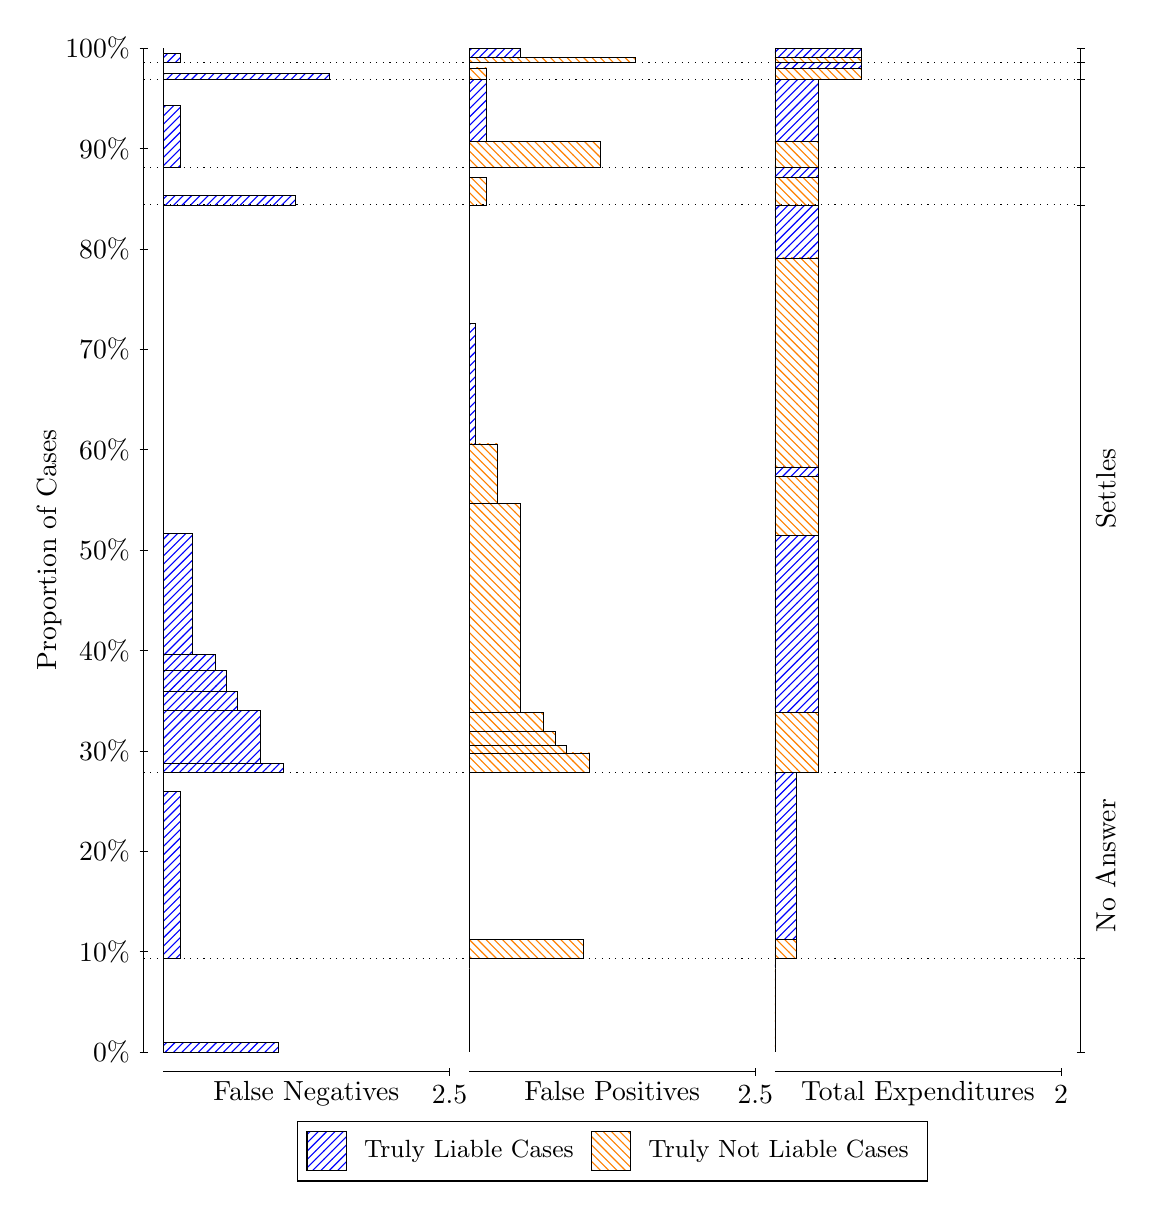
\begin{tikzpicture}
\draw[black, very thin] (1.5,1.75) -- (1.5,14.5);
\node[rotate=90, text=black, anchor=center] at (0.3, 8.125) {Proportion of Cases};
\draw[black, very thin] (1.45,1.75) -- (1.55,1.75);
\node[text=black, anchor=east] at (1.45, 1.75) {0\%};
\draw[black, very thin] (1.45,3.025) -- (1.55,3.025);
\node[text=black, anchor=east] at (1.45, 3.025) {10\%};
\draw[black, very thin] (1.45,4.3) -- (1.55,4.3);
\node[text=black, anchor=east] at (1.45, 4.3) {20\%};
\draw[black, very thin] (1.45,5.575) -- (1.55,5.575);
\node[text=black, anchor=east] at (1.45, 5.575) {30\%};
\draw[black, very thin] (1.45,6.85) -- (1.55,6.85);
\node[text=black, anchor=east] at (1.45, 6.85) {40\%};
\draw[black, very thin] (1.45,8.125) -- (1.55,8.125);
\node[text=black, anchor=east] at (1.45, 8.125) {50\%};
\draw[black, very thin] (1.45,9.4) -- (1.55,9.4);
\node[text=black, anchor=east] at (1.45, 9.4) {60\%};
\draw[black, very thin] (1.45,10.675) -- (1.55,10.675);
\node[text=black, anchor=east] at (1.45, 10.675) {70\%};
\draw[black, very thin] (1.45,11.95) -- (1.55,11.95);
\node[text=black, anchor=east] at (1.45, 11.95) {80\%};
\draw[black, very thin] (1.45,13.225) -- (1.55,13.225);
\node[text=black, anchor=east] at (1.45, 13.225) {90\%};
\draw[black, very thin] (1.45,14.5) -- (1.55,14.5);
\node[text=black, anchor=east] at (1.45, 14.5) {100\%};

\draw[black, very thin] (13.4,1.75) -- (13.4,14.5);
\draw[black, very thin] (13.35,1.75) -- (13.45,1.75);
\node[anchor=west] at (13.35, 1.75) {};
\draw[black, very thin] (13.35,2.9362) -- (13.45,2.9362);
\node[anchor=west] at (13.35, 2.9362) {};
\draw[black, very thin] (13.35,5.2999) -- (13.45,5.2999);
\node[anchor=west] at (13.35, 5.2999) {};
\draw[black, very thin] (13.35,12.508) -- (13.45,12.508);
\node[anchor=west] at (13.35, 12.508) {};
\draw[black, very thin] (13.35,12.983) -- (13.45,12.983);
\node[anchor=west] at (13.35, 12.983) {};
\draw[black, very thin] (13.35,14.105) -- (13.45,14.105);
\node[anchor=west] at (13.35, 14.105) {};
\draw[black, very thin] (13.35,14.317) -- (13.45,14.317);
\node[anchor=west] at (13.35, 14.317) {};
\draw[black, very thin] (13.35,14.5) -- (13.45,14.5);
\node[anchor=west] at (13.35, 14.5) {};

\draw[black, very thin, pattern color=blue, pattern=north east lines] (1.75,1.75) rectangle (3.2033,1.8748);
\draw[black, very thin, pattern color=orange, pattern=north west lines] (1.75,1.8748) rectangle (1.75,2.9362);
\draw[black, very thin, pattern color=blue, pattern=north east lines] (1.75,2.9362) rectangle (1.968,5.0546);
\draw[black, very thin, pattern color=orange, pattern=north west lines] (1.75,5.0546) rectangle (1.75,5.2999);
\draw[black, very thin, pattern color=blue, pattern=north east lines] (1.75,5.2999) rectangle (3.276,5.4193);
\draw[black, very thin, pattern color=blue, pattern=north east lines] (1.75,5.4193) rectangle (2.9853,6.0928);
\draw[black, very thin, pattern color=blue, pattern=north east lines] (1.75,6.0928) rectangle (2.6947,6.3341);
\draw[black, very thin, pattern color=blue, pattern=north east lines] (1.75,6.3341) rectangle (2.5493,6.5987);
\draw[black, very thin, pattern color=blue, pattern=north east lines] (1.75,6.5987) rectangle (2.404,6.8023);
\draw[black, very thin, pattern color=blue, pattern=north east lines] (1.75,6.8023) rectangle (2.1133,8.334);
\draw[black, very thin, pattern color=orange, pattern=north west lines] (1.75,8.334) rectangle (1.75,12.508);
\draw[black, very thin, pattern color=blue, pattern=north east lines] (1.75,12.508) rectangle (3.4213,12.631);
\draw[black, very thin, pattern color=orange, pattern=north west lines] (1.75,12.631) rectangle (1.75,12.983);
\draw[black, very thin, pattern color=blue, pattern=north east lines] (1.75,12.983) rectangle (1.968,13.774);
\draw[black, very thin, pattern color=orange, pattern=north west lines] (1.75,13.774) rectangle (1.75,14.105);
\draw[black, very thin, pattern color=blue, pattern=north east lines] (1.75,14.105) rectangle (3.8573,14.173);
\draw[black, very thin, pattern color=orange, pattern=north west lines] (1.75,14.173) rectangle (1.75,14.317);
\draw[black, very thin, pattern color=blue, pattern=north east lines] (1.75,14.317) rectangle (1.968,14.432);
\draw[black, very thin, pattern color=orange, pattern=north west lines] (1.75,14.432) rectangle (1.75,14.5);
\draw[black, very thin, pattern color=orange, pattern=north west lines] (5.6333,1.75) rectangle (5.6333,2.8114);
\draw[black, very thin, pattern color=blue, pattern=north east lines] (5.6333,2.8114) rectangle (5.6333,2.9362);
\draw[black, very thin, pattern color=orange, pattern=north west lines] (5.6333,2.9362) rectangle (7.0867,3.1815);
\draw[black, very thin, pattern color=blue, pattern=north east lines] (5.6333,3.1815) rectangle (5.6333,5.2999);
\draw[black, very thin, pattern color=orange, pattern=north west lines] (5.6333,5.2999) rectangle (7.1593,5.5488);
\draw[black, very thin, pattern color=orange, pattern=north west lines] (5.6333,5.5488) rectangle (6.8687,5.641);
\draw[black, very thin, pattern color=orange, pattern=north west lines] (5.6333,5.641) rectangle (6.7233,5.824);
\draw[black, very thin, pattern color=orange, pattern=north west lines] (5.6333,5.824) rectangle (6.578,6.0653);
\draw[black, very thin, pattern color=orange, pattern=north west lines] (5.6333,6.0653) rectangle (6.2873,8.7192);
\draw[black, very thin, pattern color=orange, pattern=north west lines] (5.6333,8.7192) rectangle (5.9967,9.4739);
\draw[black, very thin, pattern color=blue, pattern=north east lines] (5.6333,9.4739) rectangle (5.706,11.006);
\draw[black, very thin, pattern color=blue, pattern=north east lines] (5.6333,11.006) rectangle (5.6333,12.508);
\draw[black, very thin, pattern color=orange, pattern=north west lines] (5.6333,12.508) rectangle (5.8513,12.86);
\draw[black, very thin, pattern color=blue, pattern=north east lines] (5.6333,12.86) rectangle (5.6333,12.983);
\draw[black, very thin, pattern color=orange, pattern=north west lines] (5.6333,12.983) rectangle (7.3047,13.314);
\draw[black, very thin, pattern color=blue, pattern=north east lines] (5.6333,13.314) rectangle (5.8513,14.105);
\draw[black, very thin, pattern color=orange, pattern=north west lines] (5.6333,14.105) rectangle (5.8513,14.249);
\draw[black, very thin, pattern color=blue, pattern=north east lines] (5.6333,14.249) rectangle (5.6333,14.317);
\draw[black, very thin, pattern color=orange, pattern=north west lines] (5.6333,14.317) rectangle (7.7407,14.384);
\draw[black, very thin, pattern color=blue, pattern=north east lines] (5.6333,14.384) rectangle (6.2873,14.5);
\draw[black, very thin, pattern color=orange, pattern=north west lines] (9.5167,1.75) rectangle (9.5167,2.8114);
\draw[black, very thin, pattern color=blue, pattern=north east lines] (9.5167,2.8114) rectangle (9.5167,2.9362);
\draw[black, very thin, pattern color=orange, pattern=north west lines] (9.5167,2.9362) rectangle (9.7892,3.1815);
\draw[black, very thin, pattern color=blue, pattern=north east lines] (9.5167,3.1815) rectangle (9.7892,5.2999);
\draw[black, very thin, pattern color=orange, pattern=north west lines] (9.5167,5.2999) rectangle (10.062,6.0653);
\draw[black, very thin, pattern color=blue, pattern=north east lines] (9.5167,6.0653) rectangle (10.062,8.3065);
\draw[black, very thin, pattern color=orange, pattern=north west lines] (9.5167,8.3065) rectangle (10.062,9.0612);
\draw[black, very thin, pattern color=blue, pattern=north east lines] (9.5167,9.0612) rectangle (10.062,9.1806);
\draw[black, very thin, pattern color=orange, pattern=north west lines] (9.5167,9.1806) rectangle (10.062,11.835);
\draw[black, very thin, pattern color=blue, pattern=north east lines] (9.5167,11.835) rectangle (10.062,12.508);
\draw[black, very thin, pattern color=orange, pattern=north west lines] (9.5167,12.508) rectangle (10.062,12.86);
\draw[black, very thin, pattern color=blue, pattern=north east lines] (9.5167,12.86) rectangle (10.062,12.983);
\draw[black, very thin, pattern color=orange, pattern=north west lines] (9.5167,12.983) rectangle (10.062,13.314);
\draw[black, very thin, pattern color=blue, pattern=north east lines] (9.5167,13.314) rectangle (10.062,14.105);
\draw[black, very thin, pattern color=orange, pattern=north west lines] (9.5167,14.105) rectangle (10.607,14.249);
\draw[black, very thin, pattern color=blue, pattern=north east lines] (9.5167,14.249) rectangle (10.607,14.317);
\draw[black, very thin, pattern color=orange, pattern=north west lines] (9.5167,14.317) rectangle (10.607,14.384);
\draw[black, very thin, pattern color=blue, pattern=north east lines] (9.5167,14.384) rectangle (10.607,14.5);
\draw[black, dotted] (1.5,2.9362) -- (13.4,2.9362);
\draw[black, dotted] (1.5,5.2999) -- (13.4,5.2999);
\draw[black, dotted] (1.5,12.508) -- (13.4,12.508);
\draw[black, dotted] (1.5,12.983) -- (13.4,12.983);
\draw[black, dotted] (1.5,14.105) -- (13.4,14.105);
\draw[black, dotted] (1.5,14.317) -- (13.4,14.317);
\draw[black, very thin] (1.75,1.5) -- (5.3833,1.5);
\node[text=black, anchor=north] at (3.5667, 1.5) {False Negatives};
\draw[black, very thin] (5.3833,1.45) -- (5.3833,1.55);
\node[text=black, anchor=north] at (5.3833, 1.45) {2.5};

\draw[black, very thin] (5.6333,1.5) -- (9.2667,1.5);
\node[text=black, anchor=north] at (7.45, 1.5) {False Positives};
\draw[black, very thin] (9.2667,1.45) -- (9.2667,1.55);
\node[text=black, anchor=north] at (9.2667, 1.45) {2.5};

\draw[black, very thin] (9.5167,1.5) -- (13.15,1.5);
\node[text=black, anchor=north] at (11.333, 1.5) {Total Expenditures};
\draw[black, very thin] (13.15,1.45) -- (13.15,1.55);
\node[text=black, anchor=north] at (13.15, 1.45) {2};


\node[text=black, centered, rotate=90] at (13.72, 4.118) {No Answer};
\node[text=black, centered, rotate=90] at (13.72, 8.904) {Settles};





\draw (7.449999999999999,1.5) node[draw=none] (baseCoordinate) {};
\begin{scope}[align=center]
        \matrix[scale=0.5, draw=black, below=0.5cm of baseCoordinate, nodes={draw}, column sep=0.1cm]{
            \node[rectangle, draw, minimum width=0.5cm, minimum height=0.5cm, pattern color=blue, pattern=north east lines] {}; &
            \node[draw=none, font=\small, text=black] (B) {Truly Liable Cases}; &
            \node[rectangle, draw, minimum width=0.5cm, minimum height=0.5cm, pattern color=orange, pattern=north west lines] {}; &
            \node[draw=none, font=\small, text=black] (B) {Truly Not Liable Cases}; \\
            };
\end{scope}

\end{tikzpicture}
\end{document}